\documentclass[]{article}
\usepackage[utf8]{inputenc}
\usepackage[english,russian]{babel}
\usepackage{amsmath}
\usepackage{enumerate}
\usepackage[12pt]{extsizes}
\linespread{1.3}
\usepackage[left=3cm, top=1.5cm, right=1.3cm, bottom=2cm, nohead, footskip=10mm]{geometry}


\usepackage[absolute,overlay]{textpos}
\usepackage{indentfirst}
\usepackage{float}
\restylefloat{table}
\usepackage{hyperref}
\usepackage{mathtext}
\usepackage{amsfonts}
\usepackage{amsthm}
\usepackage{tikz}
\usepackage{xspace}
\usepackage{listings}
\usetikzlibrary{shapes,positioning,shadows,trees,automata,arrows.meta,shapes.geometric}
\usepackage{pgf-pie}
\usepackage{chngcntr}
\usepackage{pdfpages}
\usepackage{systeme}
\usepackage{empheq}
\numberwithin{equation}{section}
\usepackage{caption}
\DeclareCaptionLabelSeparator{none}{. }
\captionsetup{labelsep=none}


\pagestyle{plain}

\renewcommand{\labelenumii}{\theenumii}
\renewcommand{\theenumii}{\arabic{enumii}.}

\captionsetup[lstlisting]{
    singlelinecheck=false
    ,margin=3pt,
    font=,
    skip=5pt
    }


\lstdefinestyle{TEXTstyle}{
    basicstyle=\footnotesize\ttfamily,
    aboveskip=0pt,
	belowskip=10pt,
	showspaces=false,
	showstringspaces=false,
    basicstyle=\ttfamily\footnotesize,
    texcl=true,
    morecomment=[l]{\#},
    commentstyle=\color{gray},
    frame=tb
}

\begin{document}
    \thispagestyle{empty}
	\begin{center}
		Министерство образования и науки Российской Федерации\\
		Санкт-Петербургский политехнический университет Петра Великого \\
		Институт прикладной математики и механики\\
		Кафедра <<Телематика>>\\
		\vspace{5cm}
		\textbf{\textbf{ЛАБОРАТОРНАЯ РАБОТА}}\\
        \vspace{0.5cm}
        \textbf{ПО ТЕМЕ}\\
        \vspace{0.5cm}
		\textbf{\textbf{<<Методы кластеризации>>}}\\
		\vspace{3cm}
		по направлению 02.04.01.02 <<Организация и управление суперкомпьютерными системами>>
	\end{center}
	\vspace{2cm}
	\begin{tabular} {l l l}
	\hspace{9.5cm} & Выполнил: & \\
	& Студент гр. 13643.1 & Титов А.И.\\
	& Проверил: & Уткин Л.В.
	\end{tabular}
	\vspace{4.5cm}
	\begin{center}
		Санкт-Петербург\\
		2019
    \end{center}


	\renewcommand\contentsname{Оглавление}
	\tableofcontents

    \newpage
    \section*{Постановка задачи}
    \addcontentsline{toc}{section}{Постановка задачи}

    Требуется решить выполнить следующие задачи:

    \begin{enumerate}
        \item Разбить множество объектов из набора данных pluton в пакете «cluster» на 3 кластера методом центров тяжести (kmeans). Сравнить качество разбиения в зависимости от максимального числа итераций алгоритма.
        \item  Сгенерировать набор данных в двумерном пространстве, состоящий из 3 кластеров, каждый из которых сильно “вытянут” вдоль одной из осей. Исследовать качество кластеризации методом clara в зависимости от
            \begin{enumerate}
                \item Использования стандартизации;
                \item Типа метрики.
            \end{enumerate}
        Объясните полученные результаты.
        \item  Построить дендрограмму для набора данных votes.repub в пакете «cluster» (число голосов, поданных за республиканцев на выборах с 1856 по 1976 год). Строки представляют 50 штатов, а столбцы - годы выборов (31).
        \item Построить дендрограмму для набора данных animals в пакете «cluster». Данные содержат 6 двоичных признаков для 20 животных. Переменные:
            \begin{enumerate}
                \item war - теплокровные;
                \item fly - летающие;
                \item ver - позвоночные;
                \item end - вымирающие;
                \item gro - живущие в группе;
                \item hai - имеющие волосяной покров.
            \end{enumerate}
        \item Рассмотреть данные из файла seeds\_dataset.txt, который содержит описание зерен трех сортов пшеницы: Kama, Rosa and Canadian. Признаки:
            \begin{enumerate}
                \item область A;
                \item периметр P;
                \item компактность C = $\frac{4\pi A}{P^2}$;
                \item длина зерна;
                \item ширина зерна;
                \item коэффициент ассиметрии;
                \item длина колоска.
            \end{enumerate}
    \end{enumerate}

    \section{Набор данных <<Pluton>>}

    Для кластеризации из набора данных были выбраны только первые два признака. Данные были разбиты на 3 кластера с помощью метода k-средних. Было проведено исследование влияния параметра максимального числа итераций на разбиение. Были использованы следующие значения параметров: 1, 1000, 2000. Был построен график разбиения (Рис. 1). На рисунке представлены результаты трех разбиений по значению изменяемого параметра, соответственно. Как можно пронаблюдать - многие точки были причислены к разным кластерам в зависимости от разбиения.

    \begin{figure}[H]
        \centering
        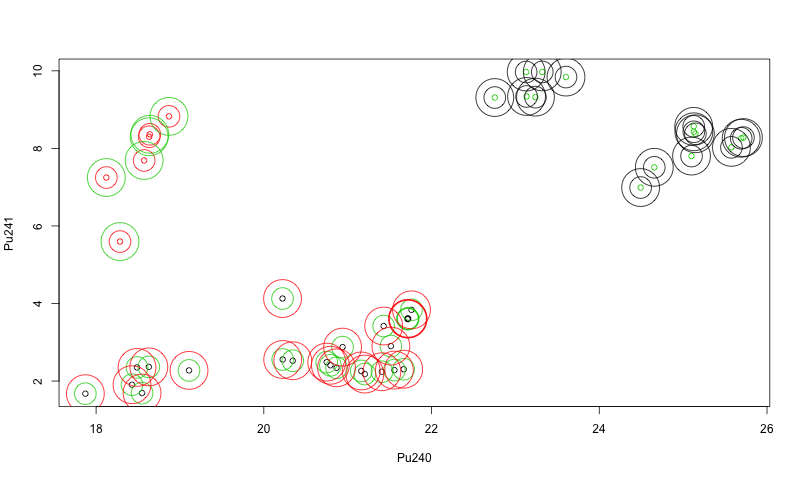
\includegraphics[width = 0.9\linewidth]{data/pluton_clustering.png}
        \caption{Кластеризация набора данных <<pluton>>}
    \end{figure}

    \section{Сгенерированный набор данных}
    Был сгенерирован набор данных, состоящий из 3ех кластеров. Каждый кластер вытянут по одной из осей. Была проведена кластеризация методом clara с использованием 2 метрик (manhattan и euclidean) и с использованием стандартизации и без нее. Кластеризация была визуализирована (Рис. 2).

    \begin{figure}[H]
        \centering
        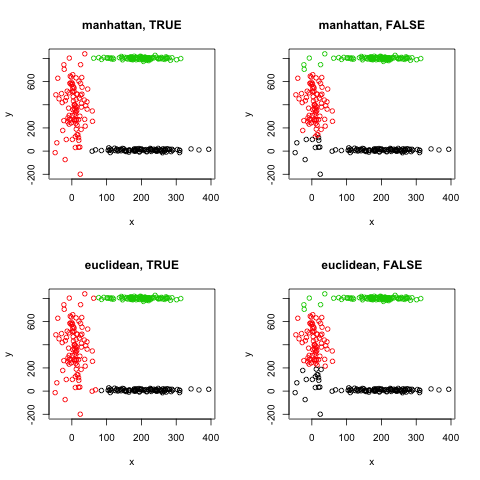
\includegraphics[width = 0.9\linewidth]{data/generated.png}
        \caption{Кластеризация сгенерированного набора данных}
    \end{figure}

    \section{Набор данных <<votes.repub>>}
    Для данного набора данных была построена дендограмма (Рис. 3), отображающая информацию о близости отдельных кластеров к друг другу и показывающая непосредственно последовательность разделения кластеров.

    \begin{figure}[H]
        \centering
        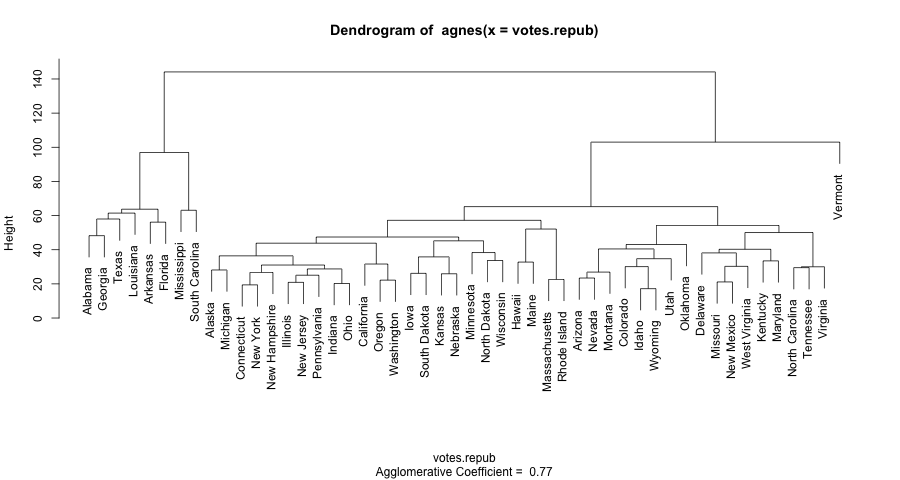
\includegraphics[width = 0.9\linewidth]{data/votes.png}
        \caption{Дендограмма для набора данных <<votes.repub>>}
    \end{figure}

    \section{Набор данных <<animals>>}

    Для набора данных была построена дендограмма (Рис. 4). Так как разбиений в данном наборе данных значительно меньше чем в предыдущем, здесь можно пронаблюдать последовательность разделения более детально.

    \begin{figure}[H]
        \centering
        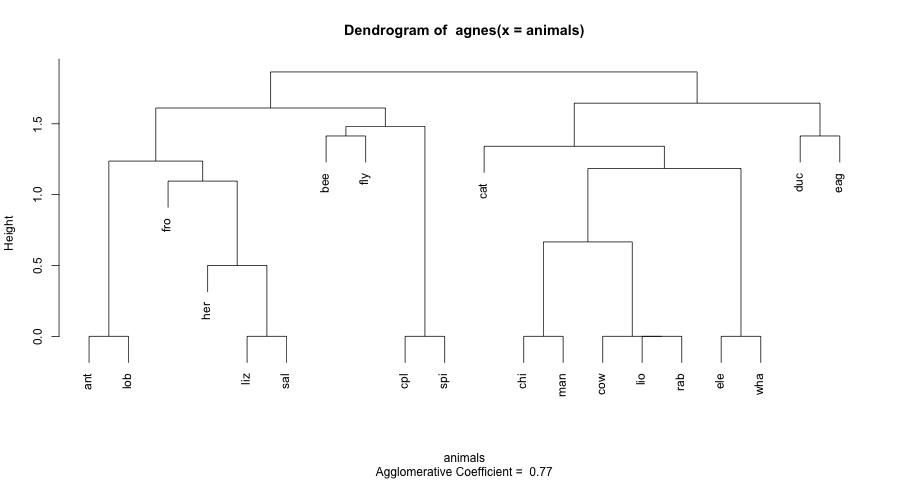
\includegraphics[width = 0.9\linewidth]{data/animals.png}
        \caption{Дендограмма для набора данных <<animals>>}
    \end{figure}

    \section{Набор данных <<seeds>>}

    Для набора данных были построены разбиения на три кластера. Разбиения представлены на Рис. 5.

    \begin{figure}[H]
        \centering
        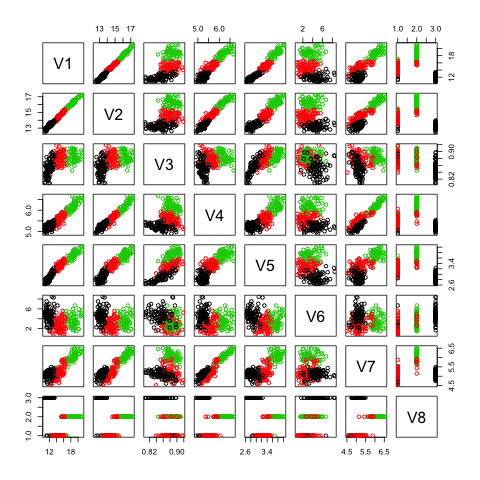
\includegraphics[width = 0.9\linewidth]{data/seeds.png}
        \caption{Кластеризация набора данных <<seeds>>}
    \end{figure}

\end{document}
